%\VignetteIndexEntry{UsingRDataTracker} 

% This file was converted to LaTeX by Writer2LaTeX ver. 1.2
% see http://writer2latex.sourceforge.net for more info

% Conversion and modifications by Luis Perez 17-Jul-2014
\documentclass[letterpaper]{article}
\usepackage[utf8]{inputenc}
\usepackage[T1]{fontenc}
\usepackage[english]{babel}
\usepackage{amsmath}
\usepackage{amssymb,amsfonts,textcomp}
\usepackage{color}
\usepackage{array}
\usepackage{hhline}
\usepackage{hyperref}
\hypersetup{pdftex, colorlinks=true, linkcolor=blue, citecolor=blue, filecolor=blue, urlcolor=blue, pdftitle=}
\usepackage[pdftex]{graphicx}
% List styles
\newcounter{saveenum}
\newcommand\liststyleWWNumxv{%
\renewcommand\theenumi{\arabic{enumi}}
\renewcommand\theenumii{\alph{enumii}}
\renewcommand\theenumiii{\alph{enumii}.\roman{enumiii}}
\renewcommand\theenumiv{\alph{enumii}.\roman{enumiii}.\arabic{enumiv}}
\renewcommand\labelenumi{\theenumi.}
\renewcommand\labelenumii{\theenumii.}
\renewcommand\labelenumiii{\theenumiii.}
\renewcommand\labelenumiv{\theenumiv.}
}
% Page layout (geometry)
\setlength\voffset{-1in}
\setlength\hoffset{-1in}
\setlength\topmargin{1in}
\setlength\oddsidemargin{1in}
\setlength\textheight{8.5398in}
\setlength\textwidth{6.5in}
\setlength\footskip{0.9602in}
\setlength\headheight{0cm}
\setlength\headsep{0cm}
% Footnote rule
\setlength{\skip\footins}{0.0469in}
\renewcommand\footnoterule{\vspace*{-0.0071in}\setlength\leftskip{0pt}\setlength\rightskip{0pt plus 1fil}\noindent\textcolor{black}{\rule{0.25\columnwidth}{0.0071in}}\vspace*{0.0398in}}
% Pages styles
\makeatletter
\newcommand\ps@Standard{
  \renewcommand\@oddhead{}
  \renewcommand\@evenhead{}
  \renewcommand\@oddfoot{\thepage{}}
  \renewcommand\@evenfoot{\@oddfoot}
  \renewcommand\thepage{\arabic{page}}
}
\makeatother
\pagestyle{Standard}
\title{}
\begin{document}
\clearpage\setcounter{page}{1}\pagestyle{Standard}
{\centering
\textbf{Using RDataTracker}
\par}

\begin{center}
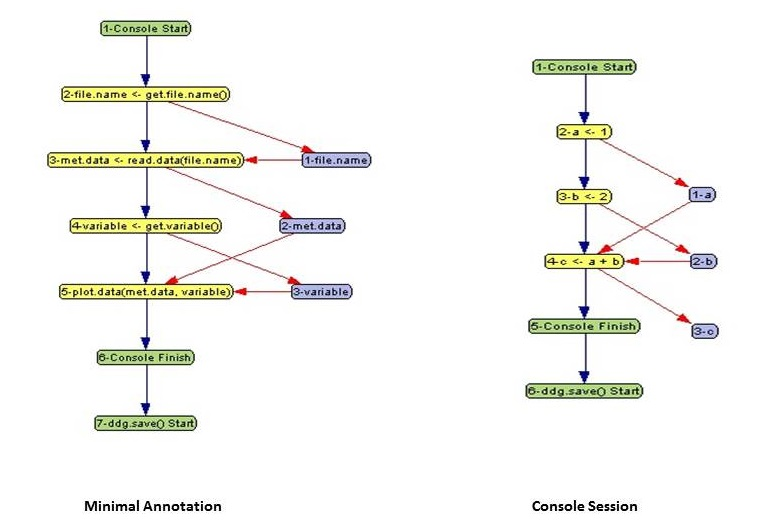
\includegraphics[width=5.4067in,height=3.7594in]{UsingRDataTracker-img/UsingRDataTracker-img001.jpg}
\end{center}
\begin{center}
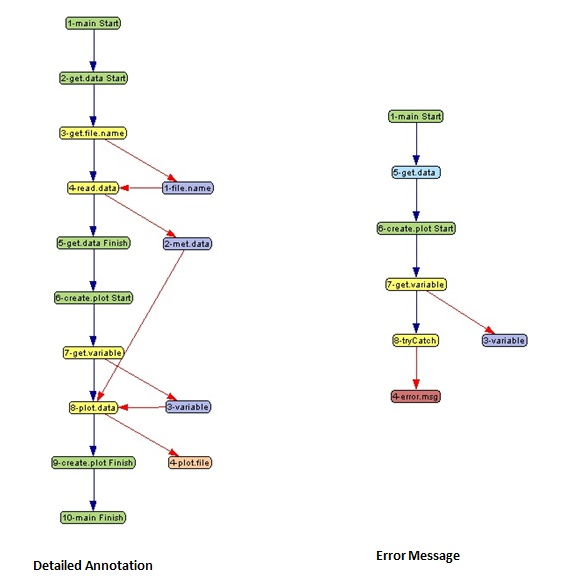
\includegraphics[width=4.4232in,height=4.5724in]{UsingRDataTracker-img/UsingRDataTracker-img002.jpg}
\end{center}
{\centering
\textbf{Emery Boose \& Barbara Lerner}
\par}

{\centering
\textbf{May 2014}
\par}


\bigskip

\liststyleWWNumxv
\begin{enumerate}
\item \textbf{What is RDataTracker?}
\end{enumerate}

\bigskip

RDataTracker is a library of R functions that can be used to annotate (instrument) an R script in order to collect data provenance in the form of a Data Derivation Graph (DDG) as the script executes. \ It can also be used to collect data provenance during R console sessions. \ RDataTracker saves the DDG as a text file (ddg.txt), with ancillary files stored in a special DDG directory. \ The DDG can then be viewed, stored, and queried using a separate tool, DDG Explorer.


\bigskip

\liststyleWWNumxv
\setcounter{saveenum}{\value{enumi}}
\begin{enumerate}
\setcounter{enumi}{\value{saveenum}}
\item \textbf{What is a DDG?}
\end{enumerate}

\bigskip

A Data Derivation Graph (DDG) is a mathematical graph that captures the history of a data analysis. \ The DDG consists of nodes and edges. \ In DDG Explorer, nodes are shown as ovals and edges are shown as arrows (see below for examples). \ Different colors (explained in the legend for DDG Explorer) are used to indicate different types of nodes and edges.


\bigskip

There are two major types of nodes---procedural nodes and data nodes---and two major types of edges---control flow edges and data flow edges. \ Control flow edges indicate how control passes from one procedural node to another procedural node as the script executes. \ Data flow edges indicate how input data pass from a data node to a procedural node or how output data pass from a procedural node to a data node.


\bigskip

Procedural nodes include Operational, Collapsible, Expandable, Checkpoint, and Restore nodes. \ Operational nodes perform an operation. \ Collapsible nodes and expandable nodes provide a level of abstraction by allowing a section of the DDG to be expanded or collapsed. \ Checkpoint nodes indicate creation of a checkpoint. \ Restore nodes indicate that a previous checkpoint was restored.


\bigskip

Data nodes include Data, File, Snapshot, URL, and Exception nodes. \ Data nodes are used for simple values. \ File nodes are used for files that are inputs to the R script or created by the R script. \ Snapshot nodes are used for complex data values such as data frames. \ URL nodes are used for URL addresses. \ Exception nodes are used for error messages. \ The values of Data, URL, and Exception nodes are stored in the DDG text file. \ The values of File and Snapshot nodes are stored as files in the DDG directory.


\bigskip

For more details on DDGs and how to view, store, and query them, please see the DDG Explorer documentation (UsingDDGExplorer.pdf).


\bigskip

\liststyleWWNumxv
\setcounter{saveenum}{\value{enumi}}
\begin{enumerate}
\setcounter{enumi}{\value{saveenum}}
\item \textbf{Installation and Use}
\end{enumerate}

\bigskip

The following instructions assume you are using RStudio. \ Example scripts are shown in blue. See section 9 for DDG examples


\bigskip

RDataTracker is distributed as an R package. \ Note that R packages must be \textit{installed} to your computer (normally just once) and then \textit{loaded} for use in a particular session.


\bigskip

To install RDataTracker, copy or download the package file to your computer, open RStudio, and use the Tools / Install Packages option to install from a Package Archive File (alternatively you can use the \textbf{install.packages} command at the R prompt). \ Once the library has been installed, select Packages / RDataTracker to see a list of help pages for the various functions. \ Note that all functions begin with \textbf{ddg.} to avoid confusion with function names in the main script.


\bigskip

To load RDataTracker, use the \textbf{library(RDataTracker)} command at the R prompt or at the top of your script. \ Alternatively you can click on the checkbox for RDataTracker in the list of packages in RStudio. \ The library needs to know the path and name of the R script itself and the path for the DDG files that will be created (see below for how to provide this information). \ We recommend creating a DDG directory separate from the working directory for each R script.


\bigskip

A DDG is created by adding function calls to RDataTracker as described below. \ Once the script is properly annotated, data provenance will be collected as the R script executes. \ This information is stored in memory and written to the DDG file (\textbf{ddg.txt}) on the DDG directory when the R script finishes. \ The DDG file contains information about the computing environment, the number of procedural steps, and the specifications for individual nodes and edges of the DDG. \ Step and data nodes are each numbered in sequence beginning with one. \ Simple data values (e.g. numbers) are stored in the DDG itself. \ More complex data values (e.g. data frames) are stored as pointers to files created on the DDG directory. \ Input and output files of the main script are stored as pointers to copies of those files created on the DDG directory. \ While the DDG file can be viewed using a text editor, its primary purpose is to support exchange of information and it should normally be viewed and queried using DDG Explorer.


\bigskip

The library functions are introduced below. \ For more details, please see the help pages under Packages / RDataTracker in RStudio.


\bigskip

\liststyleWWNumxv
\setcounter{saveenum}{\value{enumi}}
\begin{enumerate}
\setcounter{enumi}{\value{saveenum}}
\item \textbf{Minimal Annotation}
\end{enumerate}

\bigskip

A simple DDG can be created with minimal annotation of an R script, as illustrated below:


\bigskip

\textcolor[rgb]{0.21176471,0.37254903,0.5686275}{library(RDataTracker)}

\textcolor[rgb]{0.21176471,0.37254903,0.5686275}{setwd(``c:/data/r/example'')}

\textcolor[rgb]{0.21176471,0.37254903,0.5686275}{r.script.path {\textless}- paste(getwd(), ''test.r'', sep=''{}'')}

\textcolor[rgb]{0.21176471,0.37254903,0.5686275}{ddgdir {\textless}- paste(getwd(), ''/ddg'', sep=''{}'')}

\textcolor[rgb]{0.21176471,0.37254903,0.5686275}{ddg.init(r.script.path, ddgdir, enable.console=TRUE)}


\bigskip

\textcolor[rgb]{0.21176471,0.37254903,0.5686275}{\{main script\}}


\bigskip

\textcolor[rgb]{0.21176471,0.37254903,0.5686275}{ddg.save()}


\bigskip

Here the first line loads the RDataTracker package. \ The second line sets the working directory. \ The third line specifies the path and name of the R script. \ The fourth line specifies the directory where the DDG files will be stored. \ The fifth line initiates creation of a DDG. \ The sixth line saves the DDG.


\bigskip

When \textbf{enable.console} is set to TRUE, the library captures assignment statements as Operational nodes and associated data values as Data nodes. \ This approach is useful for getting a quick view of a data analysis.


\bigskip

\liststyleWWNumxv
\setcounter{saveenum}{\value{enumi}}
\begin{enumerate}
\setcounter{enumi}{\value{saveenum}}
\item \textbf{Console Sessions}
\end{enumerate}

\bigskip

A similar approach can be used to capture console sessions in R.


\bigskip

\textcolor[rgb]{0.21176471,0.37254903,0.5686275}{{\textgreater}library(RDataTracker)}

\textcolor[rgb]{0.21176471,0.37254903,0.5686275}{{\textgreater}ddg.init(ddgdir=''c:/data/r/console/ddg'', enable.console=TRUE)}


\bigskip

\textcolor[rgb]{0.21176471,0.37254903,0.5686275}{\{console commands\}}


\bigskip

\textcolor[rgb]{0.21176471,0.37254903,0.5686275}{{\textgreater}ddg.save()}


\bigskip

Here the first line loads the RDataTracker package. \ The second line initiates creation of a DDG and specifies where the DDG files will be stored. \ The third line saves the DDG. \ Note that \textbf{ddg.save} may be called more than once during a console session to add to the current DDG, while calling \textbf{ddg.init} again replaces the current DDG with a new DDG.


\bigskip

\liststyleWWNumxv
\setcounter{saveenum}{\value{enumi}}
\begin{enumerate}
\setcounter{enumi}{\value{saveenum}}
\item \textbf{Annotating an R Script}
\end{enumerate}

\bigskip

A more detailed DDG may be created by adding more annotations to the original script. \ Here \textbf{enable.console} is set to FALSE in \textbf{ddg.init} and only the annotated portions of the script appear in the DDG.


\bigskip

The basic strategy for annotating a script is described below. \ See the help files for RDataTracker for additional details on individual functions.


\bigskip

1. Data nodes for input data to the original script are created using \textbf{ddg.data}, \textbf{ddg.file}, \textbf{ddg.snapshot}, \textbf{ddg.url}, or \textbf{ddg.exception}, depending on the data type. \ If only the variable name is supplied, the library will look up its value in the current environment.


\bigskip

\textcolor[rgb]{0.21176471,0.37254903,0.5686275}{ddg.data(x)}


\bigskip

2. Operational nodes are created using \textbf{ddg.procedure}. \ If \textbf{ddg.procedure} is called from inside an R function and the name of the node is omitted, the library will use the name of the function.


\bigskip

\textcolor[rgb]{0.21176471,0.37254903,0.5686275}{ddg.procedure()}


\bigskip

3. Input data nodes are assumed to exist when \textbf{ddg.procedure} is called. \ Data flow edges to one or more existing input data nodes can be created using a list of values and the \textbf{ins} parameter of \textbf{ddg.procedure}. \ 


\bigskip

\textcolor[rgb]{0.21176471,0.37254903,0.5686275}{ddg.procedure(ins=list(``x1'', ``x2''))}


\bigskip

If \textbf{ddg.procedure} is called from inside an R function and if \textbf{lookup.ins} is set to TRUE, the library will create a data flow edge to each argument passed to the function, if a corresponding data node exists.


\bigskip

\textcolor[rgb]{0.21176471,0.37254903,0.5686275}{ddg.procedure(lookup.ins=TRUE)}


\bigskip

A data flow edge to an existing data node may also be created using \textbf{ddg.data.in}. \ The name of operational node may be omitted if \textbf{ddg.data.in }is called from within an R function.


\bigskip

\textcolor[rgb]{0.21176471,0.37254903,0.5686275}{ddg.procedure()}

\textcolor[rgb]{0.21176471,0.37254903,0.5686275}{ddg.data.in(x)}


\bigskip

4. One or more output data nodes and corresponding data flow edges may be created using a list of values and the \textbf{outs.data}, \textbf{outs.file}, \textbf{outs.snapshot}, \textbf{outs.url}, or \textbf{outs.exception} parameters of \textbf{ddg.procedure}, depending on the data type.


\bigskip

\textcolor[rgb]{0.21176471,0.37254903,0.5686275}{ddg.procedure(outs.data=list(``z1'', z2''))}


\bigskip

A single output data node and corresponding data flow edge may also be created using \textbf{ddg.data.out}, \textbf{ddg.file.out}, \textbf{ddg.snapshot.out}, \textbf{ddg.url.out}, or \textbf{ddg.exception.out}, depending on the data type. \ The name of the operational node may be omitted if \textbf{ddg.data.out}, etc is called from within an R function.


\bigskip

\textcolor[rgb]{0.21176471,0.37254903,0.5686275}{ddg.procedure()}

\textcolor[rgb]{0.21176471,0.37254903,0.5686275}{ddg.data.out(x)}


\bigskip

5. Expandable and collapsible nodes, implemented through calls to \textbf{ddg.start} and \textbf{ddg.finish}, may be used to create levels of abstraction in the DDG. \ These functions must be correctly nested with matching arguments.


\bigskip

\textcolor[rgb]{0.21176471,0.37254903,0.5686275}{ddg.start(``calculate.square.root'')}


\bigskip

\textcolor[rgb]{0.21176471,0.37254903,0.5686275}{\{intervening R code\}}


\bigskip

\textcolor[rgb]{0.21176471,0.37254903,0.5686275}{ddg.finish(``calculate.square.root'')}


\bigskip

Clicking on the start or finish node in DDG Explorer will collapse the intervening nodes to a single node, while clicking on a single collapsed node will expand to reveal the intervening nodes.


\bigskip

6. A DDG is created and saved using the \textbf{ddg.init} and \textbf{ddg.save} functions. \ The annotation is essentially the same as for the minimal DDG described above, except that \textbf{enable.console} is set to FALSE.


\bigskip

\textcolor[rgb]{0.21176471,0.37254903,0.5686275}{library(RDataTracker)}

\textcolor[rgb]{0.21176471,0.37254903,0.5686275}{setwd(``c:/data/r/example'')}

\textcolor[rgb]{0.21176471,0.37254903,0.5686275}{r.script.path {\textless}- paste(getwd(), ''test.r'', sep=''{}'')}

\textcolor[rgb]{0.21176471,0.37254903,0.5686275}{ddgdir {\textless}- paste(getwd(), ''/ddg'', sep=''{}'')}

\textcolor[rgb]{0.21176471,0.37254903,0.5686275}{ddg.init(r.script.path, ddgdir, enable.console=FALSE)}


\bigskip

\textcolor[rgb]{0.21176471,0.37254903,0.5686275}{\{main script\}}


\bigskip

\textcolor[rgb]{0.21176471,0.37254903,0.5686275}{ddg.save()}


\bigskip

Alternatively, \textbf{ddg.run} can be used instead of \textbf{ddg.init} and \textbf{ddg.save} if the main program is implanted as a single function. \ One advantage to this approach is that if an R error occurs during execution of the function, the error will be capture in an Exception node in the DDG.


\bigskip

\textcolor[rgb]{0.21176471,0.37254903,0.5686275}{library(RDataTracker)}

\textcolor[rgb]{0.21176471,0.37254903,0.5686275}{setwd(``c:/data/r/example'')}

\textcolor[rgb]{0.21176471,0.37254903,0.5686275}{r.script.path {\textless}- paste(getwd(), ''test.r'', sep=''{}'')}

\textcolor[rgb]{0.21176471,0.37254903,0.5686275}{ddgdir {\textless}- paste(getwd(), ''/ddg'', sep=''{}'')}


\bigskip

\textcolor[rgb]{0.21176471,0.37254903,0.5686275}{\{R script functions\}}


\bigskip

\textcolor[rgb]{0.21176471,0.37254903,0.5686275}{main {\textless}- function() \{}


\bigskip

\textcolor[rgb]{0.21176471,0.37254903,0.5686275}{\ \ \ \ \ \{R script main program\}}


\bigskip

\textcolor[rgb]{0.21176471,0.37254903,0.5686275}{\}}

\textcolor[rgb]{0.21176471,0.37254903,0.5686275}{ddg.run(main, r.script.path, ddgdir)}


\bigskip

\liststyleWWNumxv
\setcounter{saveenum}{\value{enumi}}
\begin{enumerate}
\setcounter{enumi}{\value{saveenum}}
\item \textbf{Checkpoint and Restore}
\end{enumerate}

\bigskip

The library contains functions that can be used to save and restore the R state and file system state, allowing a user to return to the environment present at an earlier point in the data analysis. \ \textbf{ddg.checkpoint} adds a checkpoint node and a snapshot node and returns the full path to the file containing the saved state. \ \textbf{ddg.restore} adds a restore node with an input edge from the snapshot node for the saved checkpoint file. \ A given checkpoint can be restored more than once.


\bigskip

\textcolor[rgb]{0.21176471,0.37254903,0.5686275}{checkpoint1 {\textless}- ddg.checkpoint()}


\bigskip

\textcolor[rgb]{0.21176471,0.37254903,0.5686275}{\{intervening R code\}}


\bigskip

\textcolor[rgb]{0.21176471,0.37254903,0.5686275}{restore(checkpoint1)}


\bigskip

\liststyleWWNumxv
\setcounter{saveenum}{\value{enumi}}
\begin{enumerate}
\setcounter{enumi}{\value{saveenum}}
\item \textbf{Troubleshooting}
\end{enumerate}

\bigskip

Annotation errors are generally captured by the library and stored as error nodes in the DDG. \ The same is true for error messages from the R interpreter if the \textbf{ddg.run} function is used as described above. \ These features can be useful for troubleshooting the original script and the associated annotations.


\bigskip

The \textbf{ddg.debug.on} and \textbf{ddd.debug.off} functions may be used (in a script or at the console) to turn debugging on and off. \ \ Debugging is off by default. \ When debugging is turned on, details related to creation of the DDG are displayed in the console as the script executes.


\bigskip

The contents of the current DDG directory (if different from the working directory) may be deleted by calling the \textbf{ddg.flush.ddg} function at the R prompt.


\bigskip

\liststyleWWNumxv
\setcounter{saveenum}{\value{enumi}}
\begin{enumerate}
\setcounter{enumi}{\value{saveenum}}
\item \textbf{Acknowledgements}
\end{enumerate}

{\mdseries\upshape\color{black}
This material is based upon work supported by the National Science Foundation under Awards No. CCR-0205575, CCR-0427071, and IIS-0705772, the National Science Foundation REU grants DBI-0452254 and DBI-1003938, the Mount Holyoke Center for the Environment Summer Leadership Fellowships, and the Charles Bullard Fellowship in Forest Research at the Harvard Forest. Any opinions, findings, and conclusions or recommendations expressed in this material are those of the authors and do not necessarily reflect the views of the National Science Foundation, \ Mount Holyoke College or Harvard University.}

{\mdseries\upshape\color{black}
Numerous students have been involved in the research and tool development through the REU program at Harvard Forest. They are Shay Addams (2013 REU), Vasco Carinhas (2013 REU), Xiang Zhao (University of Massachusetts, Amherst), Luis Antonio Perez (2014 REU), Nicole Hoffler (2014 REU) .}


\bigskip

\liststyleWWNumxv
\setcounter{saveenum}{\value{enumi}}
\begin{enumerate}
\setcounter{enumi}{\value{saveenum}}
\item \clearpage
\textbf{DDG Examples}
\end{enumerate}

\bigskip

{\centering  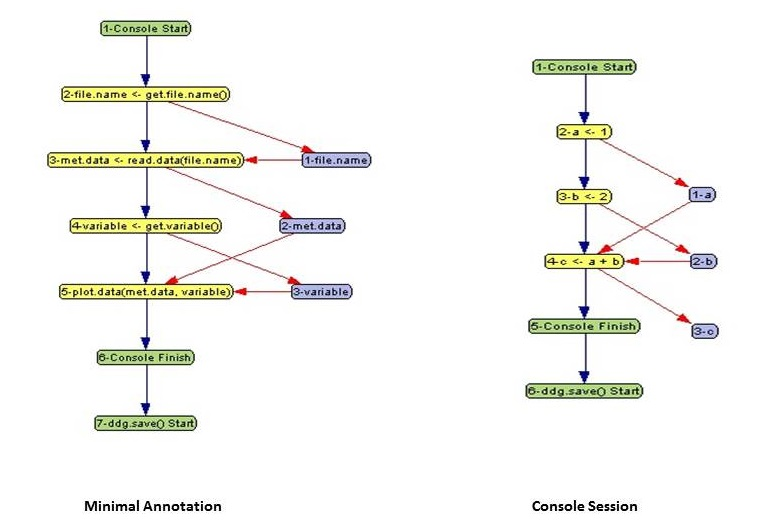
\includegraphics[width=5.4in,height=3.7547in]{UsingRDataTracker-img/UsingRDataTracker-img003.jpg} \par}

\bigskip

{\centering  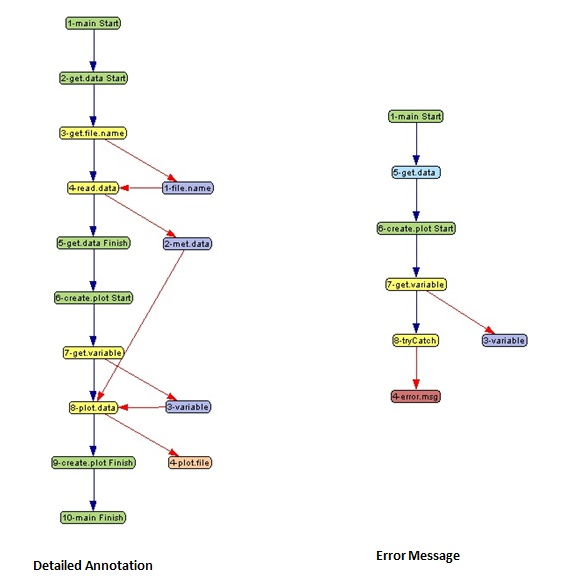
\includegraphics[width=4.4252in,height=4.5744in]{UsingRDataTracker-img/UsingRDataTracker-img004.jpg} \par}
\liststyleWWNumxv
\setcounter{saveenum}{\value{enumi}}
\begin{enumerate}
\setcounter{enumi}{\value{saveenum}}
\item \textbf{Technical Details}
\end{enumerate}

\bigskip

\textbf{Syntax of DDG Text File:}


\bigskip

{\textless}DDG{\textgreater} -{\textgreater} {\textless}Attributes{\textgreater}*{\textless}PinCounter{\textgreater} {\textless}Declaration{\textgreater}*

{\textless}Declaration{\textgreater} -{\textgreater}~ {\textless}EdgeDecl{\textgreater} {\textbar} {\textless}NodeDecl{\textgreater}~

{\textless}EdgeDecl{\textgreater} -{\textgreater} {\textless}ControlFlowDecl{\textgreater} {\textbar} {\textless}DataFlowDecl{\textgreater}

{\textless}ControlFlowDecl{\textgreater} -{\textgreater} {\textless}CF\_TOKEN{\textgreater} {\textless}ProcedureNodeID{\textgreater}{\textless}ProcedureNodeID{\textgreater}

{\textless}DataFlowDecl{\textgreater} -{\textgreater} {\textless}DF\_TOKEN{\textgreater} {\textless}DataFlowEdgeDecl{\textgreater}

{\textless}DataFlowEdgeDecl{\textgreater} -{\textgreater} {\textless}DataNodeID{\textgreater}{\textless}ProcedureNodeID{\textgreater} {\textbar} {\textless}ProcedureNodeID{\textgreater}{\textless}DataNodeID{\textgreater}

{\textless}NodeDecl{\textgreater} -{\textgreater} {\textless}DataNode{\textgreater} {\textbar} {\textless}ProcedureNode{\textgreater}

{\textless}ProcedureNode{\textgreater} -{\textgreater} {\textless}ProcedureNodeType{\textgreater} {\textless}ProcedureNodeID{\textgreater} {\textless}NAME{\textgreater}{\textquotedbl};{\textquotedbl}

{\textless}ProcedureNodeType{\textgreater} -{\textgreater} ``Operation'' {\textbar} ``Start'' {\textbar} ``Finish'' {\textbar} ``Interm'' {\textbar} ``Leaf'' {\textbar} ``SimpleHandler'' {\textbar} ``VStart'' {\textbar}

\ \ {}``VFinish'' {\textbar} ``VInterm''

{\textless}DataNode{\textgreater} -{\textgreater} {\textless}DataNodeType{\textgreater} {\textless}DataNodeID{\textgreater} {\textless}NAME{\textgreater} [{\textquotedbl}Value{\textquotedbl} {\textquotedbl}={\textquotedbl}{\textless}Value{\textgreater} ] [{\textquotedbl}Time{\textquotedbl} {\textquotedbl}={\textquotedbl} {\textless}Timestamp{\textgreater} ]

[``Location'' ``='' {\textless}FILENAME{\textgreater}] {\textquotedbl};{\textquotedbl}

{\textless}DataNodeType{\textgreater} -{\textgreater} ``Data'' {\textbar} ``Exception'' {\textbar} {\textquotedbl}URL{\textquotedbl} {\textbar} {\textquotedbl}File{\textquotedbl} {\textbar} ``Snapshot''

{\textless}Value{\textgreater} -{\textgreater} {\textless}URL{\textgreater} {\textbar} {\textless}FILENAME{\textgreater} {\textbar} {\textless}STRING{\textgreater}

{\textless}Timestamp{\textgreater} -{\textgreater} {\textless}YEAR{\textgreater}{\textquotedbl}-{\textquotedbl}{\textless}MONTH{\textgreater}{\textquotedbl}-{\textquotedbl}{\textless}DATE{\textgreater}[{\textquotedbl}T{\textquotedbl}{\textless}HOUR{\textgreater}{\textquotedbl}:{\textquotedbl}{\textless}MINUTE{\textgreater}[{\textquotedbl}:{\textquotedbl}{\textless}SECOND{\textgreater} [{\textquotedbl}.{\textquotedbl}{\textless}FRACTIONAL{\textgreater}]]]

{\textless}Attributes{\textgreater} -{\textgreater}{\textless}NAME{\textgreater}[{\textquotedbl}={\textquotedbl}]{\textless}AttrValue{\textgreater}

{\textless}AttrValue{\textgreater} -{\textgreater} {\textless}STRING{\textgreater}

{\textless}PinCounter{\textgreater} -{\textgreater} {\textless}INT{\textgreater}

{\textless}DataNodeID{\textgreater} -{\textgreater} `d' {\textless}INT{\textgreater}

{\textless}ProcedureNodeID{\textgreater} -{\textgreater} `p' {\textless}INT{\textgreater}

{\textless}CF\_TOKEN{\textgreater} -{\textgreater} ``CF''

{\textless}DF\_TOKEN{\textgreater} -{\textgreater} ``DF''


\bigskip
\end{document}
